\documentclass[10pt,xcolor=svgnames]{beamer} %Beamer
\usepackage{palatino} %font type
\usepackage{xcolor}
\usepackage[font={tiny}]{caption}
\usefonttheme{metropolis} %Type of slides
\usefonttheme[onlymath]{serif} %font type Mathematical expressions
\usetheme[progressbar=frametitle,titleformat frame=smallcaps,numbering=counter]{metropolis} %This adds a bar at the beginning of each section.
\useoutertheme[subsection=false]{miniframes} %Circles in the top of each frame, showing the slide of each section you are at

\usepackage{appendixnumberbeamer} %enumerate each slide without counting the appendix

\definecolor{SysBlue}{RGB}{12,120,183}
\definecolor{Progress}{RGB}{56,60,92}
\definecolor{Header}{RGB}{12,120,183}
\definecolor{SlideTitle}{RGB}{0,137,208}
\definecolor{ToC}{RGB}{51,58,66}

\setbeamercolor{progress bar}{fg=Progress} %These are the colours of the progress bar. Notice that the names used are the svgnames
\setbeamercolor{title separator}{fg=SysBlue} %This is the line colour in the title slide
\setbeamercolor{structure}{fg=black} %Colour of the text of structure, numbers, items, blah. Not the big text.
\setbeamercolor{normal text}{fg=black!87} %Colour of normal text
\setbeamercolor{alerted text}{fg=DarkRed!60!Gainsboro} %Color of the alert box
\setbeamercolor{example text}{fg=ToC} %Colour of the Example block text
\setbeamercolor{background canvas}{bg=white}


\setbeamercolor{palette primary}{bg=SlideTitle, fg=white} %These are the colours of the background. Being this the main combination and so one. 
\setbeamercolor{palette secondary}{bg=Header, fg=white}
\setbeamercolor{palette tertiary}{bg=Header, fg=white}
\setbeamercolor{section in toc}{fg=ToC} %Color of the text in the table of contents (toc)

%These next packages are the useful for Physics in general, you can add the extras here. 
\usepackage{amsmath,amssymb}
\usepackage{slashed}
\usepackage{cite}
\usepackage{relsize}
\usepackage{caption}
\usepackage{subcaption}
\usepackage{multicol}
\usepackage{booktabs}
\usepackage[scale=2]{ccicons}
\usepackage{pgfplots}
\usepgfplotslibrary{dateplot}
\usepackage{geometry}
\usepackage{xspace}
\usepackage{enumitem}
\newcommand{\themename}{\textbf{\textsc{bluetemp}\xspace}}%metropolis}}\xspace}

\title{Pachira Fund}
\author[Name]{Ian Moore, PhD \inst{$\dagger$}}%With inst, you can change the institution they belong
\subtitle{Can Money Grow on Trees?}

\institute[shortinst]{\inst{$\dagger$} Tokenomics Researcher / Engineer @ Syscoin (email: imoore@syscoin.org) }

\date{November 13, 2023} %Here you can change the date
\titlegraphic{\vspace{-0.5cm}\hfill
\includegraphics[scale=0.23]{logo.png}} %You can modify the location of the logo by changing the command \vspace{}. 

\begin{document}
{
\setbeamercolor{background canvas}{bg=white, fg=black}
\setbeamercolor{normal text}{fg=black}
\maketitle
}%This is the colour of the first slide. bg= background and fg=foreground

\metroset{titleformat frame=smallcaps} %This changes the titles for small caps

\begin{frame}{Outline}
  \setbeamertemplate{section in toc}[sections numbered] %This is numbering the sections
  \tableofcontents[hideallsubsections] %You can comment this line if you want to show the subsections in the table of contents
\end{frame}

\begin{frame}{Objectives}

\metroset{block=fill}
\begin{exampleblock}{\textsc{First ever smart DAO protocol}}
\begin{itemize}
  \item Similar to Ethereum in the sense that both protocols work with decentralized immutable storage
  \item Instead launching contracts from chains, we work with Diamonds
\end{itemize}  
\end{exampleblock}

\begin{exampleblock}{\textsc{Self-sovereign capital coordination}}
\begin{itemize}
  \item Does this via its new Autonomous Service Engine technology
  \item Made possible through an extension of the multi-facet proxy called Diamonds outlined in EIP-2535
\end{itemize}
\end{exampleblock}

\begin{exampleblock}{\textsc{Masternode Yield Farming}}
\begin{itemize}
  \item First of a new class of DAOs
  \item System of trustlessly investing Masternode yields into a DeFi liquidity provider
\end{itemize}
\end{exampleblock}

\end{frame}


\section{Introduction}

\begin{frame}{Introduction: Overview} %You can change fragile by standout

slide

\end{frame}


\section{What are we Solving?}

\begin{frame}{Stagnant Pool Problem} 

slide

\end{frame}


\begin{frame}{Uniswap v3} 

\begin{figure}[h!]
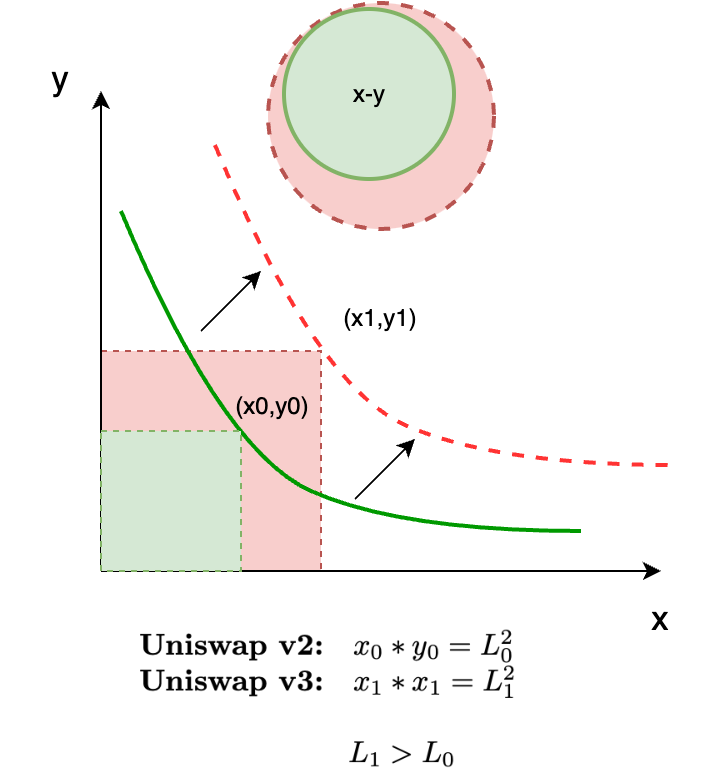
\includegraphics[width=2.3in]{img/uniswap_v3.png}
\caption{Uniswap v3} 
\label{fig:uniswap_v3}
\end{figure}

\end{frame}

\begin{frame}{Indexing Problem} 

slide

\end{frame}


\begin{frame}{Simple Tree} 

\begin{figure}[h!]
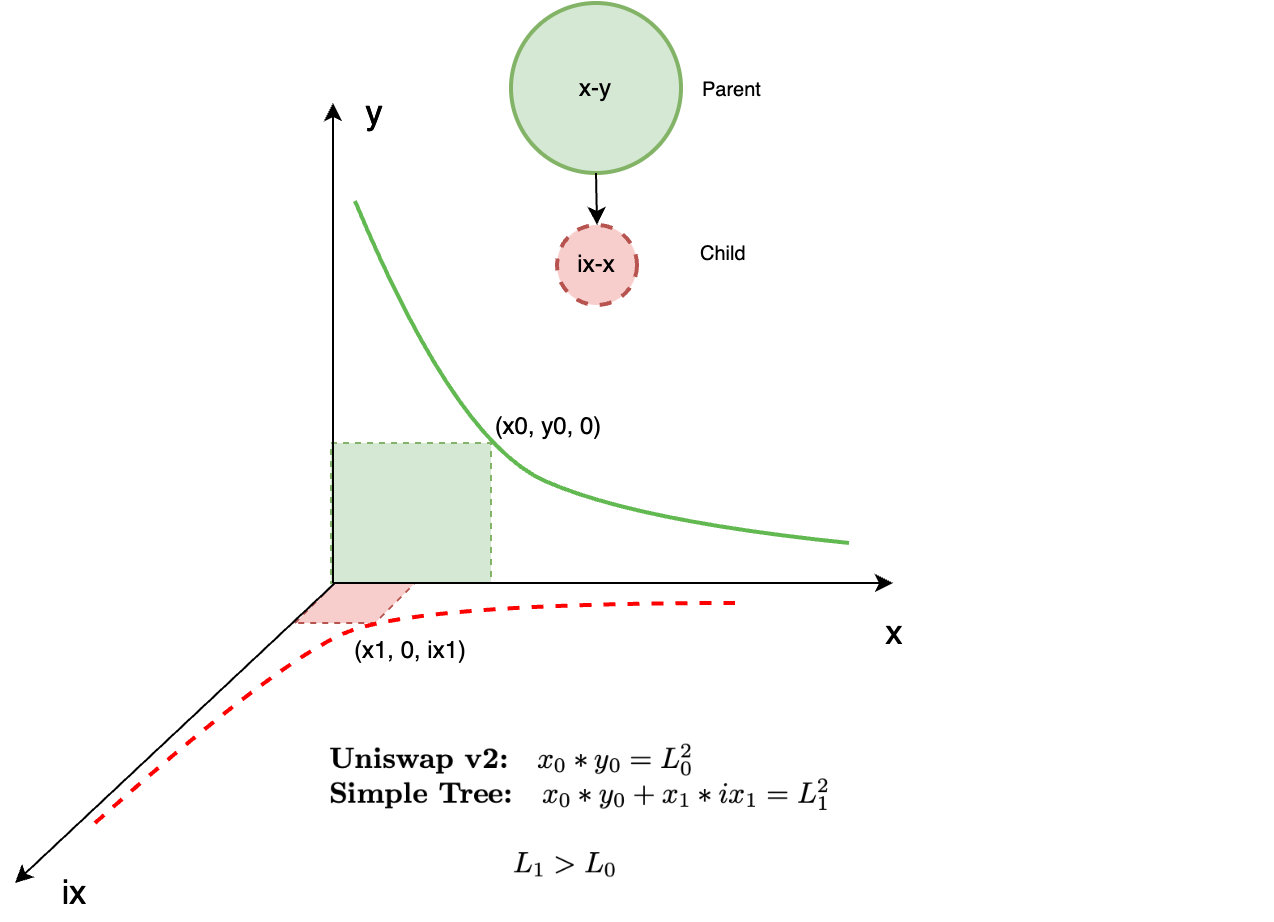
\includegraphics[width=3in]{img/simple_tree.png}
\caption{Simple Tree} 
\label{fig:simple_tree}
\end{figure}

\end{frame}

\begin{frame}{How does this Work?} 

\begin{figure}[h!]
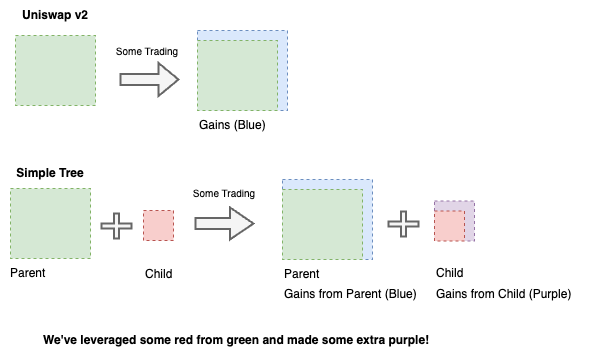
\includegraphics[width=3in]{img/compare.png}
\caption{Comparison} 
\label{fig:compare}
\end{figure}

\end{frame}



\section{Liquidity Trees}

\begin{frame}{Full Tree} 

\begin{figure}[h!]
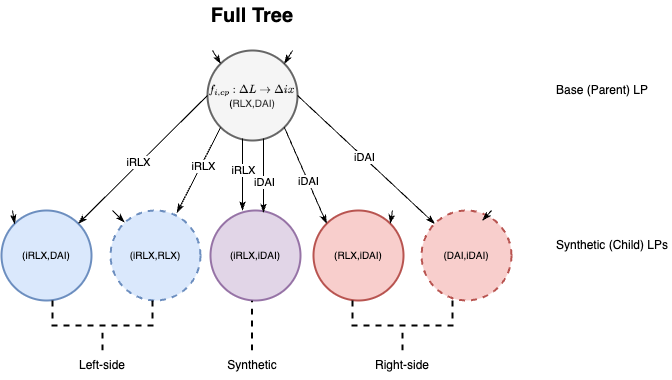
\includegraphics[width=3in]{img/full_tree.png}
\caption{Full Tree} 
\label{fig:full_tree}
\end{figure}

\end{frame}

\begin{frame}{Sub Trees} 

\begin{figure}[h!]
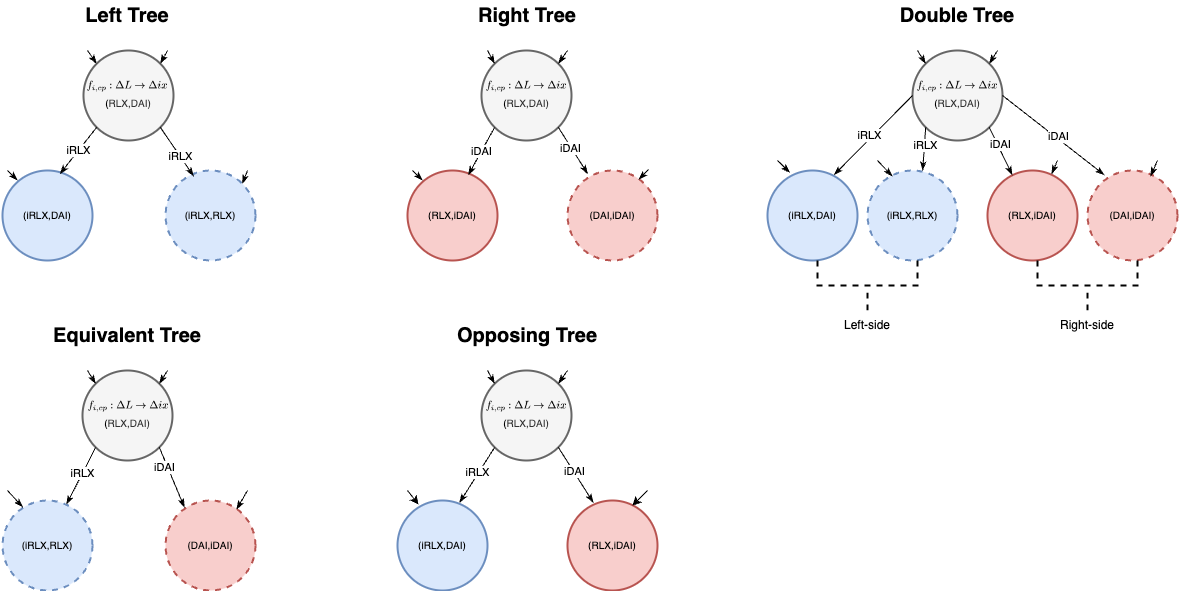
\includegraphics[width=3in]{img/sub_trees.png}
\caption{Sub Tree} 
\label{fig:sub_trees}
\end{figure}

\end{frame}


\section{Simulation Results}

\begin{frame}{Left Tree}

\begin{figure}[h!]
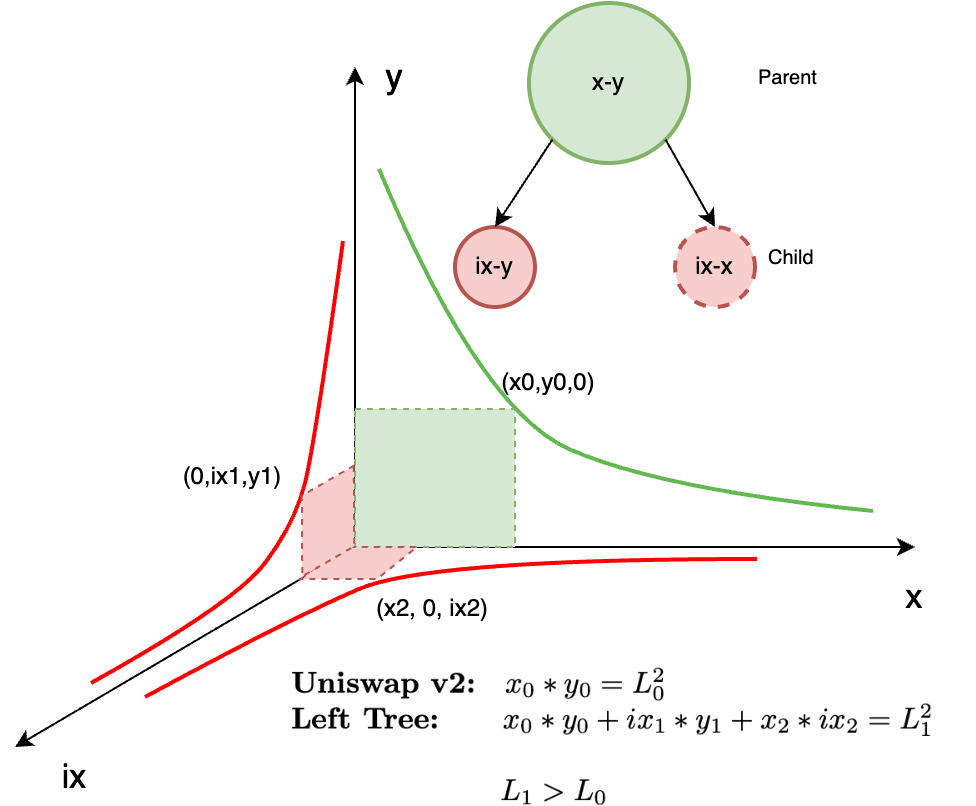
\includegraphics[width=3in]{img/left_tree.png}
\caption{Left Tree} 
\label{fig:left_tree}
\end{figure}

\end{frame}


\begin{frame}{Price action}

slide

\end{frame}


\begin{frame}{Revenue Chart}

slide

\end{frame}


\begin{frame}{Revenue Table}

slide

\end{frame}


\section{Revist our Hypothesis}

\begin{frame}{Tokenomics: General Model}

slide

\end{frame}






\begin{frame}[standout]
  Thank you! 
\end{frame}



\end{document}